\documentclass{article}

\usepackage{pdfcomment}
\usepackage[margin=1in]{geometry}
\usepackage{xcolor}
\usepackage{graphicx}

\newcommand{\note}[2]{\pdfmargincomment[color=yellow,author=#1,open=true]{#2}}
\newcommand{\todo}[1]{\color{red}\textbf{TODO:}#1\color{black}}

\title{Numerical error propagation in the HCP structural pre-processing pipelines}

\author{M. Ali Salari, Lalet Scaria, Gregory Kiar, Lindsay B. Lewis,
  Alan C. Evans, Tristan Glatard}

\begin{document}

\maketitle

\abstract{This paper is a reproducibility study of the work in~\cite{glasser2015multi}.}

\section{Introduction}

Operating systems are known to have an effect on the results produced
by neuroimaging pipelines~\cite{Gronenschild2012, Glatard2015},
presumably due to the creation, propagation and amplification of small
numerical errors across the pipelines.  Such errors highlight
numerical instability which is also likely to appear as a result of
other types of small perturbations such as acquisition and parametric
noise. However, the precise causes of
such instabilities and the path along which they propagate in the
pipelines are unclear.  We present a technique to identify the
processes in a pipeline that create numerical errors along the
execution, and we apply this technique to the HCP structural
pre-processing pipelines.


Groenschild \emph{et al.} first identified the effect of operating
systems on Freesurfer
results~\cite{Gronenschild2012}. In~\cite{10.3389/fninf.2015.00012} we
quantified this effect on some of the main neuroimaging pipelines
including several FSL pipelines, CIVET and Freesurfer. In this work we
aim at evaluating this effect on the work in~\cite{glasser2015multi}.
\todo{Link this to Lindsay's HBM 2017 poster and to Redolfi et al.}

The operating system is defined here as a consistent set of software
packages organized in a trusted repository.

The operating system is not the only part of the computational
environment that may hamper reproducibility. The work
in~\cite{diethelm2012limits} mentions reproducibility issues coming
from parallelization.

Notes:
\begin{itemize}
  \item Reproducibility has several other aspects, see, e.g.,
\url{https://medium.com/@lorenaabarba/barba-group-reproducibility-syllabus-e3757ee635cf#.ty3zmgd4k}
 \item James P Turner, speaker in INCF 2016 Track B, is looking at numerical stability on GPUs. And reproducibility.
 \item For an overview of variability accross analysis methods in fMRI, see \url{http://journal.frontiersin.org/article/10.3389/fnins.2012.00149/full}.
 \item For a general overview in fMRI, see \url{http://www.nature.com/nrn/journal/vaop/ncurrent/box/nrn.2016.167_BX3.html}
\end{itemize}
   
\section{Materials and Methods}

\subsection{Data and Processing}

We randomly selected 10 subjects from the HCP data release S500 and processed them on a 
containerized version of HCP pipelines. The Docker images are built for the HCP structural 
pre-processing pipelines v3.19.0 (PreFreeSurfer and FreeSurfer)~\cite{Glasser2013} 
in CentOS 6.8 and CentOS 7.2 for the ease of conducting the experiment and reproducibility issues. 
We collected the provenance trace (tree of executed processes and files accessed in read or write mode) 
for one subject using system-call interception as provided by the reprozip tool~\cite{5}.

\subsection{HCP Minimal preprocessing Pipelines}

The Human Connectom Project (HCP)~\cite{Gla13} is a set of pipelines To help extraction of structural, functional or diffusion MRI data
across a large set of high resolution MR images.these preprocessing pipelines creates results that are available in standard
volume and combined surface and volume spaces which makes it easier for researchers to compare
the images across the neuroimaging spectrum.

\paragraph{Structural Pipelines} The structural pre-processing consists of PreFreeSurfer, FreeSurfer and PostFreeSurfer. 
\paragraph{Functional Pipelines} Functional pre-processing consists of fMRIVolume and fMRISurface~\cite{FSL}. 
\paragraph{Diffusion Preprocessing pipeline} preparing...

\paragraph{Processing environment}

To ensure that the origin of differences are generated exactly across the operating system updates (inter-os differences) 
on HCP preprocessing pipelines, some pre-executions have been done in a wrapper script; 
(a) the checksum of the files are computed in each subject before and after a multiple execution to detect 
potential intra-condition differences (e.g., use of pseudo-random numbers). 
(b) Checksum of Docker container is recorded to make sure that the same container was used all over. Also, list of packages 
with versions is printed for every task. (c) Hardware information is captured to make sure that differences are not coming from, for instance, different CPUs (when on cluster).

HCP preprocessing pipelines are both time-consuming and computationally intensive which might even run for days, depending upon 
the type and size of dataset. We made use of a web platform (CBRAIN) for managing the containers and data with the help of Boutiques technology. 
The Canadian Brain Imaging Research Platform (CBRAIN), is a web platform developed at the Montreal Neurological Institute (MNI) to tackle 
the Big-Data research and heavy computational challenges faced by neuroimaging researchers. ~\cite{DBLP:journals/fini/DasGRSPMSRSKMKR17}.
CBRAIN supports container technologies like Docker, Singularity and it also extends its support to Boutiques. Thus, 
with the help of container technologies and Boutiques, applications can be ported to CBRAIN. Any user who has access to this application 
can try to reproduce the experiments since the data and the application are accessible within the framework. However, one caveat is that, 
the neuroimaginng pipelines might have different results due to differences in computing platforms on which the images are getting processed ~\cite{10.3389/conf.fninf.2014.18.00076}
therefore, the execution results of the pipelines across different operating systems are considered to find out 
the cause of the reproducibility issues using an interposition techniques for the provenance capture.


\begin{itemize}
  \item monitor.sh - For monitoring the hardware details and software library versions
  \item create-execution.sh for keeping the input directories unmodified and thus preventing modification of input files.
  \item checksums.sh - To make sure that the files are not corrupted while transferring or processing the subjects.
  \item command-line-script.sh - For submitting the PreFreeSurfer Pipeline script with the right paramets.
  \item command-line-script.sh - For submitting the PreFreeSurfer Pipeline script with the right paramets.
  \item Checksums to detect file corruption.
  \item Hardware information is captured to make sure that differences are not coming from, e.g., different CPUs (when on cluster).
  \item Checksum of Docker container is recorded to make sure that the same container was used all over. Also, list of packages with versions is printed for every task. 
  \item Multiple runs are executed per condition to detect potential intra-condition differences (e.g., use of pseudo-random numbers).
\end{itemize}

\subsection{Measuring differences}

We computed a file difference matrix between files produces in each operating system based on file checksum as in~\cite{Scaria2017}.
 The checksums are computed before and after execution so that corruption check can be done with the use of recorded checksums.
 We have used MD5 {\url{https://tools.ietf.org/html/rfc1321}} algorithm for calculating the checksum of files. 
The output of a MD5 algorithm is a 128-bit ``fingerprint" or ``message digest"~\cite{md5}. 
Though MD5 is not completely secure against collision attack, Repro-tools focus more on the data integrity than security 
and how fast the algorithm is able to create the checksum. These qualities make MD5 a good choice for checksum generation in Repro-tools.
\paragraph{} For the files that are identified to have differences, different kind of metrics are used base on the file 
type to quantify the differences. Normalized root mean square error, Dice Coefficient, Text filter etc. are the 
various metrics used for quantifying the differences. As defined in \cite{khosrow2017handbook}, ``The Root Mean Square Deviation (RMSD) 
or root-mean-square error (RMSE) is a frequently used measure of the difference between values predicted by a model or 
an estimator and the values actually observed". Normalizing the RMSD value makes it easier to compare between models or datasets.
\paragraph{} Dice Similarity Coefficient can be used as a statistical validation metric for measuring the reproducibility
 of magnetic resonance images~\cite{Zou2004}. To measure the similarity of image files in reproducibility study, we used dice similarity coefficient. 
The coefficient ranges from 0.0 to 1. 1 meaning the images are exactly similiar and 0 meaning there is zero similarity.
\paragraph{} These metric values help us understand how big or small the differences are. Apart from quantifying 
the differences using type specific metrics, Repro-tools can also be used to trace the provenance of these differences.
 It is able to identify all the processes and associated parameters that wrote the files having differences. 
These details about various processes is helpful in debugging the pipelines. This information helps in 
recreating the processing step by step and also to identify the processes that creates the differences.


Binary and non-binary.

Describe the scripts that will be written to compare results.

Describe how metrics (distances?) are associated to file types (based
on regexp) and used to compute distance matrices. Including metrics to
implement the safeguards. Report comparison algorithm (see Google
Drive).


\subsection{Pipeline analysis: Characterizing differences}

Once differences between conditions are quantified, we automatically identify the steps in the pipeline responsible for such differences.
 we use the reprozip tool [Chirigati, 2016] to record: (1) the tree of processes executed by the pipeline and
 (2) the list of files read and written by each process. This information is collected by system call interceptions, 
through the ptrace system call in Unix-like operating system, and stored in a sqlite database. The database has three 
tables including table of processes to store information of all the processes which are created by clone() 
or fork() Linux system calls and the table of opened files which keeps the detail of all files including the pipeline 
and temporary files. This table has an attribute to specify the file mode, namely files with mode 0X01 and 0X02 are read 
from and written on respectively; the final table indicated the executed files in the pipeline through execv() system call.
 In fact, the tree of processes is retrieved by query the root process at the first level and then all its child processes with 
dependency files in the next levels from database. The process tree of two subjects has tested in the same pipeline conditions
 which are similar, so we collect such data only for one subject (The term condition refers to the variation of operating systems
 on which the data processing takes place). Furthermore, the process tree is acyclic “with the respect of this assumption that 
there is no race conditions between processes to write on the same file.”
\paragraph{} In the next step, we classify the processes into three categories considering to the obtained process tree 
and the error matrix file. First, processes that read file(s) without error but write different file(s) create error in 
the pipeline. The second group of the processes are those which remove errors in pipeline, read file(s) with error and
 write “nothing or” file(s) without error. Most of the processes are in the third category beyond any fault which
 read and write file(s) without error. The processes in each category may read or write temporary file(s) that implies 
the uncertainty of the process.
\paragraph{} Pipeline is conducted of a bunch of processes sequentially, setting a modification step after classification
 of processes iteratively enables us to control the propagation of errors in the pipeline correctly. In each iteration
 we detect all the processes which are create error in the pipeline and then by fixing those processes artificially, 
we’ll find the other processes in the pipeline that introduce an error. This procedure will be terminated by fixing all the processes. 
To fix the processes that create error, we replace their dependency files with error by the same file copy from the results 
obtained in the other operating system. In this way, we were able to pinpoint the origin of the errors measured in the pipeline.

\section{Results}

Show lists of packages used with version. Focus on important
differences (e.g.: python interpreter, gcc if relevant) and explain
why these packages are important.

Show results of the comparison.

\subsection{Inter-OS differences}


\paragraph{Binary differences}


Among the 117 data files produced by PreFreeSurfer, 21 did not have any error for any subject, 92 had errors 
for all subjects and 4 had errors for 3 subjects only. 

In a previous study~\cite{Scaria2017}, we showed that
pre-processing pipelines of the Human Connectome
Project~\cite{Glasser2013} were sensitive to operating system
variation (see Figure \ref{fig:1}).
\begin{figure}
%  \includegraphics{brain\_classification}
  \caption{Tissue classification produced by the HCP pre-processing
    pipelines on subject 105216 (CentOS 6 vs CentOS 7). \todo{Represent this in a different way.}}
  \label{fig:1}
\end{figure}

\paragraph{}
Two types of differences can occur in the subjects due to the differences in the operating systems. 
One is inter-OS difference caused by the operating system library updates and the other type,
 intra-OS differences occurs as a result of the pseudo-random processes used in the pipelines.
 An example of a pseudo-random process function is, a random number generator that would get initialized 
using a seed state. the proposed method can be used to identify both kind of differences. 
The files that are common to all the subjects only are taken into consideration for comparison. The first step
 is identification of files with differences in their checksums. This is identified using the checksums that are
 recorded after the processing. Intra-OS differences are identified using the run-number added as the suffix for
 the conditions. For example, the two batches of subjects processed under the same condition (CentOS6) are stored 
as run-1 and run-2. The files belonging to the subjects stored under the above mentioned conditions are treated as intra-OS runs.



\subsection{Pipeline analysis}

Figure \ref{fig:2} shows the annotated provenance graph of the
PreFreeSurfer pipeline executed on CentOS6 and CentOS7.  Processes
that created errors are shown in red, processes that removed errors
are in blue, and other processes are in green.  Squares denote
processes for which the classification is uncertain, due to temporary
files that were removed during the execution. Black edges link
sub-processes to their parents while dashed edges denote file
dependencies between processes (green edges: files with no errors; red
edges: files with errors; yellow edges: temporary files).  The
processes that introduce errors in PreFreeSurfer are: linear
registration with “\emph{FLIRT}” (8 occurrences, in ACPC Alignment,
BrainExtraction, DistortionCorrection, AtlasRegistration), non-linear
registration with “\emph{FNIRT}” (3 occurrences, in BrainExtraction
and AltasRegistration), image warping with “\emph{new\_invwarp}” (3
occurrences, in BrainExtraction and AtlasRegistration).  In addition,
errors were observed in image mean and standard-deviation computations
with “\emph{fslstats}” (3 occurrences in BiasFieldCorrection), and in
masked image extrapolation with “\emph{fslmaths}” (1 occurrence, in
BiasFieldCorrection).  Besides, transformation format conversion with
“\emph{convertwarp}” (2 occurrences, in DistortionCorrection) was able
to remove errors.

\todo{Check if a given file is written by only one process (add a safeguard in your code).}

\begin{figure}
  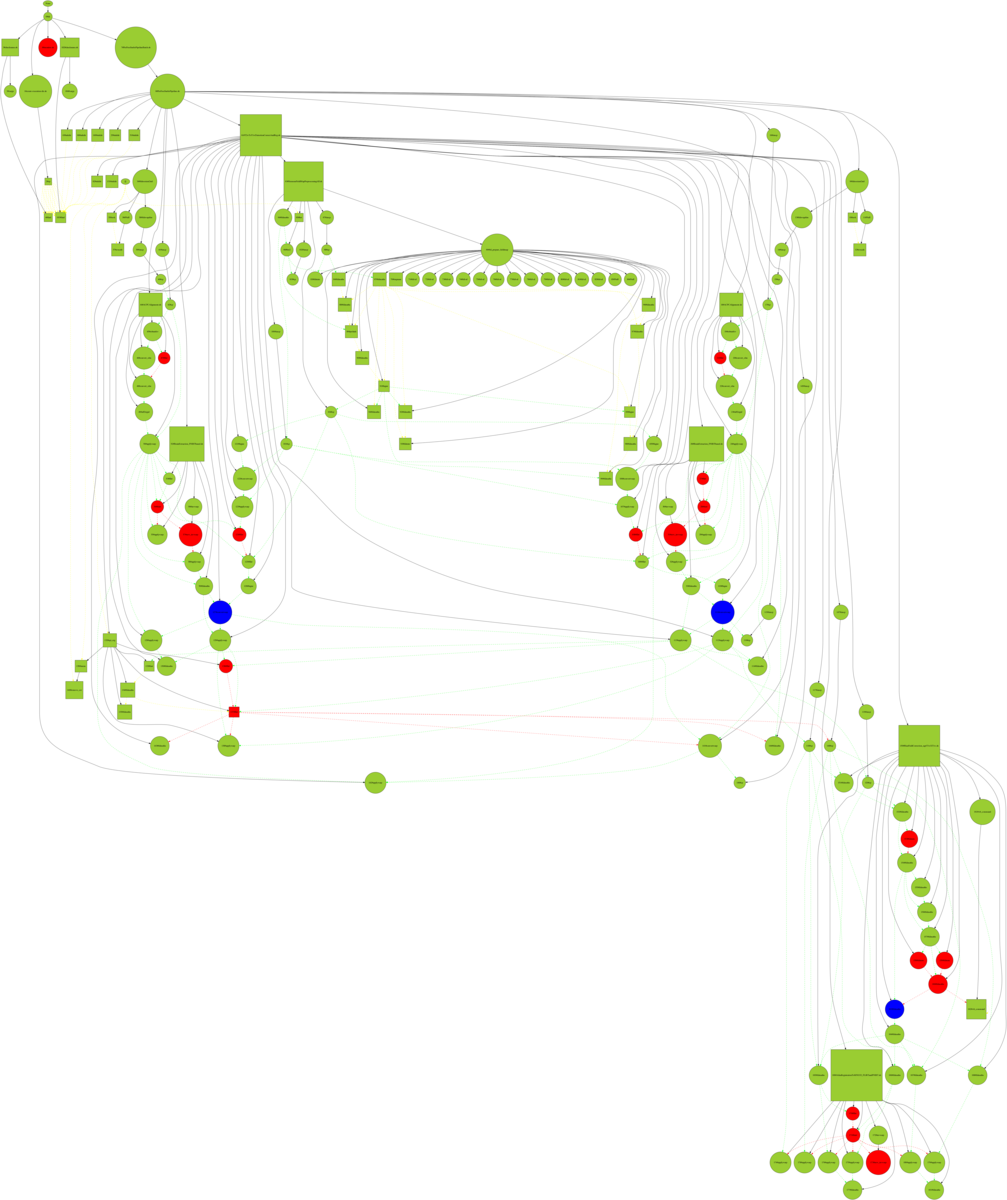
\includegraphics[width=\linewidth]{images/graph}
  \caption{An annotated provenance graph from the PreFreesurfer pipeline. Processes that created errors are in red. 
Full-resolution image available at \url{https://drive.google.com/open?id=174yyn8SuVOUcK5aRVw0bagjDanLD0FLt}.}
  \label{fig:2}
\end{figure}

\section{Discussion}

Discuss the results.

Mention that this was only possible because the unprocessed data was shared in the first place.

DICOM to Nifti conversion was out of scope and may introduce other issues.

\section{Conclusion}

Conclude and highlight future work.

The numerical instability in the PreFreesurfer HCP pipeline arises mainly from linear and non-linear registration processes 
implemented in FSL FLIRT and FNIRT. These processes need to be reviewed to understand and correct the cause of instabilities. 
In this correction process, accuracy has to be considered in addition to stability. Our technique is able to 
characterize the stability of a pipeline’s components automatically, but it also suffers from limitations as it cannot deal with: 
(1) results that are not written to disk (values processed in memory); (2) temporary files (3) files that are written by more than one process.


\section{Acknowledgments}

CBRAIN team. Compute Canada(Calcul Quebec).

\bibliographystyle{plain}
\bibliography{biblio}

\end{document}
